\documentclass[12pt]{article}

\usepackage[utf8]{inputenc}
\usepackage[portuguese]{babel}
\usepackage{indentfirst}
\usepackage{amsmath}
\usepackage{hyperref}
\usepackage[numbers,super]{natbib}
\usepackage{graphicx}
\usepackage{geometry}

\geometry{
	paper = a4paper,
    inner = 3cm,
    outer = 3cm,
    bindingoffset = .5cm,
    top = 2cm,
    bottom = 2cm
}

\begin{document}

% Title page
\begin{titlepage}
\begin{center}

\textbf{\LARGE Universidade Federal de Alagoas } \\[0.5cm]
\textbf{\large Instituto de Computação - IC}\\[0.2cm]

\vspace{20pt}

\vspace{20pt}
\vspace{20pt}
\vspace{20pt}
\vspace{20pt}
\vspace{20pt}
\vspace{20pt}
\vspace{20pt}
\vspace{20pt}

\textbf{\Large Aluno: Danilo Fernandes Costa}\\
\vspace{70pt}
\textbf{\LARGE Relatório de acopanhamento de pesquisa}\\
\vspace{20pt}
\textbf{\Large Análise e processamento de imagens PolSAR}\\
\vspace{70pt}
\textbf{\large Orientador: Alejandro Frery}\\

\vspace{45pt}
\end{center}

\par
\vfill
\begin{center}
\textbf{Maceió - AL}\\
\textbf{2018}
\end{center}

\end{titlepage}

\newpage

\section{Introdução}

Imagens PolSAR (\textit{Polarimetric Synthetic Aperture Radar}) são obtidas por meio da projeção da matriz de covariância em um espaço de cores. Contudo, como este é tridimensional, faz-se necessário uma redução de dimensionalidade, visto que, a matriz de covariância pertence a um espaço complexo de dimensão nove.

Considere a seguinte matriz de covariância:

\[
z = 
\begin{bmatrix}
	S_{\text{HH}}^{\text{*}}S_{\text{HH}} & S_{\text{HH}}^{\text{*}}S_{\text{HV}} & S_{\text{HH}}^{\text{*}}S_{\text{VV}}\\
    S_{\text{HV}}^{\text{*}}S_{\text{HH}} & S_{\text{HV}}^{\text{*}}S_{\text{HV}} & S_{\text{HV}}^{\text{*}}S_{\text{VV}}\\
    S_{\text{VV}}^{\text{*}}S_{\text{HH}} & S_{\text{VV}}^{\text{*}}S_{\text{HV}} & S_{\text{VV}}^{\text{*}}S_{\text{VV}}\\
\end{bmatrix},
\]
onde $[\cdot]^{\text{*}}$ denota o complexo conjugado. Dentre os muitos mapeamentos possíveis, um bastante comum consiste em associar diretamente os elementos $S_{\text{HH}}^{\text{*}}S_{\text{HH}}$, $S_{\text{HV}}^{\text{*}}S_{\text{HV}}$ e $S_{\text{VV}}^{\text{*}}S_{\text{VV}}$ de $z$, os quais são reais e representam a intensidade do sinal de cada uma das polarizações\cite{Frery15}, às bandas RGB, respectivamente.

Outro mapeamento possível é por meio da decomposição de Pauli, o qual associa os seguintes valores:
\begin{center}
$S_{\text{HH}}^{\text{*}}S_{\text{HH}} + S_{\text{VV}}^{\text{*}}S_{\text{VV}}$, \\
$|$ $S_{\text{VV}}^{\text{*}}S_{\text{VV}} - S_{\text{HH}}^{\text{*}}S_{\text{HH}}$ $|$, \\
$2S_{\text{HV}}^{\text{*}}S_{\text{HV}}$ \\

\end{center}
às bandas \textit{Red}, \textit{Green} e \textit{Blue}, respectivamente. Essa forma de mapear $z$ no espaço das cores, possui a característica relevante de produzir uma imagem cujas regiões encombertas por vegetação apresentam tonalidade verde.

No presente relatório, serão utilizados os mapeamentos apresentados anteriormente para obtenção de imagens a partir de dados PolSAR obtidos em \href{https://uavsar.jpl.nasa.gov}{UAVSAR} nos formatos MLC e GRD. Além disso, tendo em vista a frequência com que realiza-se processamento de quantidades volumosas de dados para a obtenção dessas imagens, será também descrita biblioteca raster e algumas disponíveis em R destinadas a Big Data que possivelmente venham a ser utéis.

\section{Descrição dos formatos MLC e GRD}

A fim de reduzir o \textit{speckle}\cite{Deng17}, o dado PolSAR é usualmente representado por matrizes de coerência de amostras de vários aspectos (\textit{multi-looked sample coherency matrices}), onde cada matriz passará a representar um pixel e é dada por:
\begin{align*}
C &= \frac{1}{N}\sum_{i = 1}^{N} z_\text{i},
\end{align*}
onde $z_\text{i}$ é uma matriz de covariância e $N$ é o número de observações para a média.

Partindo disto, temos que os arquivos MLC (\textit{Calibrated Multi-looked Cross Products}) referentes a uma certa imagem PolSAR, em conjunto, representam essas matrizes onde a média, usualmente, é de 3 pixels em \textit{range} e 12 em \textit{azimuth}. 

Tais matrizes são repartidas entre esses arquivos de modo que cada um conterá os valores correspondentes a uma das posições. Desse modo, faz-se necessário apenas seis arquivos, visto que $C$ é hermetiana. Três destes são de valores de ponto flutuante real e três de valores de ponto flutuante complexo, onde cada valor é representado por 4 bytes naqueles e 8 bytes nestes.

Além disso, os arquivos MLC são arquivos binários puros sem cabeçalho, a projeção de seus dados é a de alcance inclinado natural e o espaçamento, em metros, entre os pixels nas direções \textit{range} e \textit{azimuth} é fornecido em um arquivo de anotação junto aos mesmos.

Os arquivos GRD consistem na projeção dos dados \textit{multi-looked} no solo em coordenadas geográficas simples (latidude e longitude). No que diz respeito a quantidade dos mesmos, tipo de valor que cada um contém e número de bytes por valor, assemelham-se aos arquivos MLC. Além disso, o sistema de coordenadas é equiangular, cuja a quantidade de graus por pixel e as coordenadas do pixel do canto esquerdo superior, o qual é o de referência, são fornecidos em um arquivo de anotação.

Além do mais, em ambos os formatos a unidade dos dados é \textit{linear radar power} e possuem ordenação dos bytes \textit{little endian}, ou seja, em um tipo de dado representado por múltiplos bytes, o byte mais significativo é o último. De todo modo, a documentação desses formatos está disponível em \href{https://uavsar.jpl.nasa.gov/science/documents/polsar-format.html}{UAVSAR}.

\section{Visualização de imagens PolSAR}

As imagens visualizadas foram da cidade de Traunstein, Bayern, Alemanha e da região de Mojave, Califórnia, EUA, onde o dado PolSAR do primeiro foi proveniente de um arquivo \href{https://uavsar.jpl.nasa.gov/cgi-bin/product.pl?jobName=trauns_22551_15087_016_150604_L090_CX_01#data}{MLC} e do segundo, um arquivo \href{https://uavsar.jpl.nasa.gov/cgi-bin/product.pl?jobName=mmmmoj_18030_17050_005_170519_PL09043020_XX_01#data
}{GRD}.

Para carregar no R os arquivos MLC necessários basta executar o seguinte:
\begin{verbatim}
file_HHHH <- file("MLC_Data/HHHH.mlc", "rb")
file_HVHV <- file("MLC_Data/HVHV.mlc", "rb")
file_VVVV <- file("MLC_Data/VVVV.mlc", "rb")
\end{verbatim}

Considerando que os arquivos estão salvos em uma pasta chamada MLC\textunderscore Data no mesmo diretório daquele definido como \textit{workspace} do R e que o argumento ``rb'' passado para a função determina leitura de arquivo binário. Para o caso dos arquivos GRD, diferirá necessariamente apenas a extensão do arquivo.

A seguinte função recebe um arquivo, um número de linhas e um de colunas e retorna uma matriz com as dimensões passadas como parâmetro e preenchida sequencialmente com valores contidos no arquivo passado. 

\begin{verbatim}
read_file <- function(file, nrow, ncol) {

  return( matrix(
            readBin(file, double(), n = nrow * ncol, 
                      size = 4, endian = "little"), 
            nrow = nrow, ncol = ncol, byrow = TRUE) )
}
\end{verbatim}
A função readBin lê de arquivos binários, onde o segundo argumento é o objeto que determina o tipo do dado que será lido, o terceiro é o número elementos a serem lidos, o quarto é o número bytes por elemento e o último, a ordenação dos bytes do arquivo. 

Para visualizar a imagem PolSAR, executa-se inicialmente a função fill\textunderscore matrix, a qual receberá os arquivos contendo os dados PolSAR referentes a diagonal da matriz de coerência \textit{multi-looked}, o número de linhas e colunas da imagem e retornará uma matriz que contém as três matrizes obtidas a partir desses arquivos por meio da função read\textunderscore file.

\begin{verbatim}

fill_matrix <- function(file_HHHH, file_HVHV, file_VVVV, nrow, ncol) {
  
  amplitude_matrix <- array(0, dim = c(nrow, ncol, 3))
  amplitude_matrix[,,1] <- read_file(file_HHHH, nrow, ncol)
  amplitude_matrix[,,2] <- read_file(file_HVHV, nrow, ncol)
  amplitude_matrix[,,3] <- read_file(file_VVVV, nrow, ncol)
  
  return(amplitude_matrix) 
}
\end{verbatim}

Em posse da matriz retornada por fill\textunderscore matrix, deve-se equalizar os dados contidos na mesma, o que é feito pela seguinte função:

\begin{verbatim}
equalize <- function(data, nrow, ncol){
  
  data[,,1] <- matrix(ecdf(data[,,1])(data[,,1]), nrow = nrow, ncol = ncol)
  
  data[,,2] <- matrix(ecdf(data[,,2])(data[,,2]), nrow = nrow, ncol = ncol)
  
  data[,,3] <- matrix(ecdf(data[,,3])(data[,,3]), nrow = nrow, ncol = ncol)  
  
  return(data)
}
\end{verbatim}

A função equalize estabelecerá uma função de distribuição acumulada empírica para cada uma das matrizes que compõem aquela passada como parâmetro, por meio da função ecdf, e a aplicará no seu respectivo conjunto de dados. Após a equalização, para obter-se uma visualização dos dados PolSAR por um mapeamento direto da matriz de covariância no espaço das cores, basta executar o seguinte:

\begin{verbatim}
 writePNG(equalized_amplitude_matrix, target = "Images/mlc_image.png")
\end{verbatim}

Por meio desse processamento, obteve-se as seguintes imagens a partir dos arquivos GRD e MLC:

\begin{figure}[!ht]
	\begin{center}
		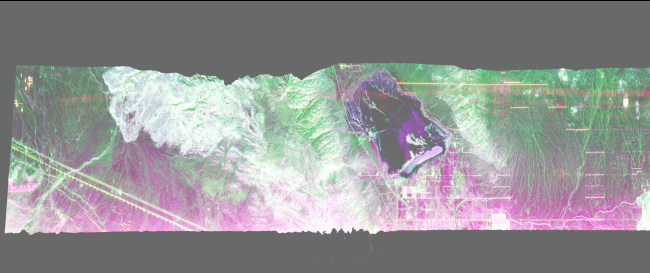
\includegraphics[width = 120mm, scale = 0.5]{../../Images/Report_07_18/grd_image_low_resolution} \\ 
        Mojare, Califórnia, EUA\\
	\end{center}
\end{figure}

\begin{figure}[!ht]
	\begin{center}
		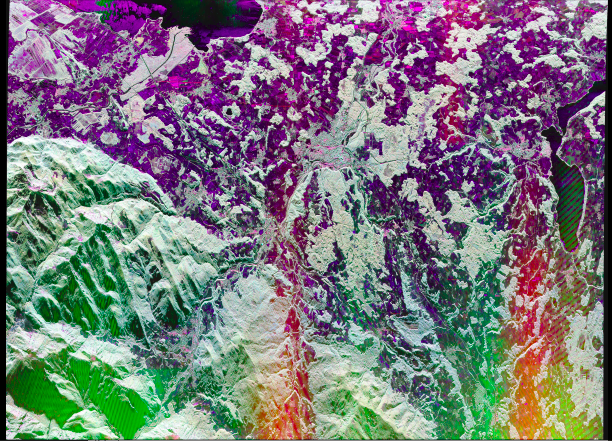
\includegraphics[width = 120mm, scale = 0.5]{../../Images/Report_07_18/mlc_image_low_resolution} \\ 
        Traunstein, Bayern, Alemanha\\
	\end{center}
\end{figure}
Outra forma de gerar uma visualização das imagens é por meio da decomposição de Pauli, a qual é obtida quando a matriz com as amplitudes das polarizações retornada pela função fill\textunderscore matrix é passada como paramétrico para a função abaixo e a matriz retornada por esta é equalizada e gerada a imagem por meio de writePNG, como mostrado acima.

\begin{verbatim}
pauli_decomposition <- function(amplitude_matrix, nrow, ncol){

  pauli_matrix <- array(0, dim = c(nrow, ncol, 3))
  pauli_matrix[,,1] <- amplitude_matrix[,,1] + amplitude_matrix[,,3]
  pauli_matrix[,,2] <- abs( amplitude_matrix[,,3] - amplitude_matrix[,,1] )
  pauli_matrix[,,3] <- 2 * amplitude_matrix[,,2]
  
  return(pauli_matrix)
}
\end{verbatim}
Seguem os resultados do processo descrito acima:
\begin{figure}[!ht]
	\begin{center}
		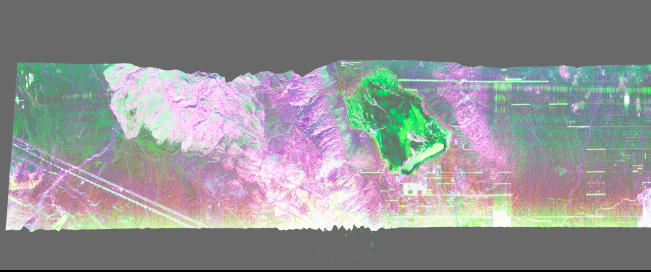
\includegraphics[width = 120mm, scale = 0.5]{../../Images/Report_07_18/grd_pauli_image_low_resolution} \\ 
        Mojare, Califórnia, EUA\\
	\end{center}
\end{figure}

\begin{figure}[!ht]
	\begin{center}
		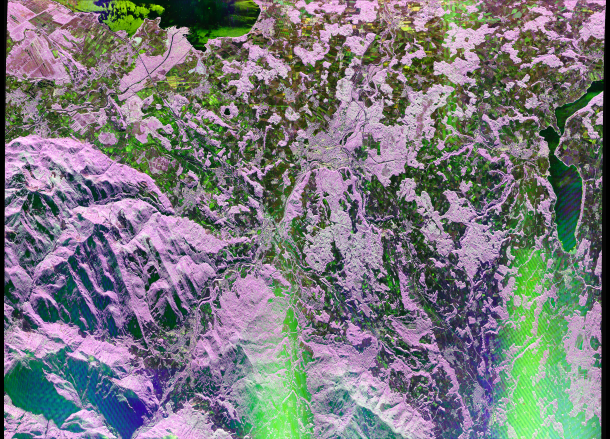
\includegraphics[width = 120mm, scale = 0.5]{../../Images/Report_07_18/mlc_pauli_image_low_resolution} \\ 
        Traunstein, Bayern, Alemanha\\
	\end{center}
\end{figure}

\section{Bibliotecas destinadas a Big Data disponíveis no R}

\subsection{Projeto Bigmemory}

O projeto Bigmemory consiste em um conjunto de bibliotecas que implementam matrizes massivas e provêm suporte para a manipulação e exploração destas. Para cada uma dessas matrizes é criada uma estrutura de dados em C++, onde permanecerão todos seus os dados, e no objeto R referente a matriz é armazenado apenas um ponteiro que aponta para a essa estrutura. Esta, por padrão, é armazenada na memória compartilhada, permitindo que processos separados compartilhem o acesso a uma única cópia do conjunto de dados.

Contudo, também é possível apoiar essa estrutura em arquivos armazenados no disco rígido e mapeados na memória, permitindo manipular grandes conjuntos de dados que excedem a capacidade da memória RAM disponível e compartilhá-los ao longo de nós em um cluster.

Esse projeto é constuído das bibliotecas bigmemory, biganalytics, bigalgebra, bigtabulate e synchronicity.

\subsubsection{Biblioteca bigmemory}

Consiste no cerne do projeto Bigmemory. Seguem algumas funções:

\begin{itemize}
\item \textbf{big.matrix}: Cria um objeto big.matrix, o qual é uma matriz segundo a especificação do Projeto Bigmemory.
\item \textbf{as.big.matrix}: Cria um objeto big.matrix a partir de uma matriz, vetor ou data.frame.
\item \textbf{as.matrix}: Converte um objeto big.matrix em uma matriz.
\item \textbf{dim}: Retorna as dimensões de uma big.matrix.
\item \textbf{flush}: Para objetos big.matrix apoiados em arquivos, essa função força as modificações realizadas a serem escritas no arquivo de apoio.
\item \textbf{read.big.matrix}: Cria uma big.matrix a partir de um arquivo formatado de acordo com o padrão ASCII. 
\item \textbf{write.big.matrix}: Escreve o conteúdo de uma big.matrix em um arquivo.
\end{itemize}

\subsubsection{Biblioteca biganalytics}

Extende a biblioteca bigmemory com funcionalidades analíticas que vão de sumários estatísticos a regressão linear. Algumas destas podem ser usadas em matrizes nativas do R para obter ganhos em velocidade e uso eficiente de memória. Seguem algumas funções:

\begin{itemize}
\item \textbf{apply}: Função análoga a nativa do R, contudo, destinada a big.matrix.
\item \textbf{bigglm.big.matrix}: Realiza regressão linear com base no conjunto de dados armazenado em uma big.matrix.
\item \textbf{bigkmeans}: Análoga a função kmeans nativa do R.
\end{itemize}

\subsubsection{Biblioteca bigalgebra}

Permite a realização de operações matriciais básicas com big.matrix com a mesma sintaxe dessas destinadas a matrizes nativas, i.e. A + B, onde A e B são objetos do tipo big.matrix.

\subsubsection{Biblioteca bigtabulate}

Extende a biblioteca bigmemory com as funcionalidades bigtable, bigsummary e bigsplit destinadas a objetos big.matrix, as quais são análogas table, summary e split nativas do R, respectivamente. Essas funcionalidades também são aplicáveis a matrizes nativas.

\subsubsection{Biblioteca synchronicity}
Provê suporte para sincronização entre processos via \textit{mutexes} e pode eventualmente suportar ipc e \textit{message passing}.\\

\textbf{Conclusões sobre o Projeto Bigmemory}\\

O Projeto Bigmemory apresenta uma abordagem de manipulação de grandes matrizes de dados de forma otimizada em relação a tempo de execução e uso de memória. Além disso, o projeto objetivou prover todas as funcionalidades existentes para as matrizes nativas do R e foi desenvolvido visando ser utilizado com programação paralela, a qual é suportada por bibliotecas já existentes no R, como Rmpi, snow, foreach e multicore.

\subsection{Biblioteca ff}

A biblioteca ff provê estruturas para que conjuntos de dados sejam armazenadas no disco rígido e possam comportar-se como se estivessem na memória RAM, por meio de mapeamento transparente na memória principal. Tem-se que os objetos ff, os quais são os principais nessa biblioteca, armazenam os dados em arquivos planos binários em codificação nativa, os quais são referenciados no R por meio de seus metadados. Além disso, arquivos ff podem ser compartilhados por múltiplos objetos ff no mesmo processo ou múltiplos processos R a fim de explorar o paralelismo. Seguem algumas funcionalidades:

\begin{itemize}
\item \textbf{ff}: Cria um objeto ff, o qual pode ser inicializado com uma matriz passando como parâmetros um vetor de dados e as dimensões da mesma.
\item \textbf{update}: Atualiza um objeto ff com o conteúdo de outro.
\item \textbf{ffapply}: Análoga a função apply nativa do R, contudo, para objetos ff.
\item \textbf{delete}: Deleta o arquivo ff pertinente a um objeto ff, sem remover este.
\item \textbf{open.ff}: Abre um arquivo ff.
\item \textbf{bigsample}: Realize amostragem a partir de um objeto ff.
\item \textbf{ffsort}: Ordena um vetor ff (um objeto ff inicializado com um vetor).
\item \textbf{length}: Tanto retorna quanto define o tamanho de um objeto ff.
\item \textbf{ffdf}: Cria um ff data.frame armazenado no disco rígido muito similar ao data.frame.
\end{itemize}

\textbf{Conclusões sobre a biblioteca ff}\\

Apresenta funcionalidades para manipulação de grandes volumes de dados sem exaurir a memória principal. Contudo, trabalha a baixo nível e não possui uma grande variedade de funções para análise dos dados.


\section{Biblioteca raster}

A biblioteca raster provê funcionalidades destinadas a manipulação de dados geográficos. Esses dados são trabalhados dentro de objetos Raster, onde o espaço é dividido em células de igual tamanho, cujas unidades estarão no sistema de coordenadas de referência. 

Além do mais, essa biblioteca suporta o uso de \textit{datasets} volumosos que não podem ser carregados inteiramente na memória principal. Isso é possível, pois suas funções podem carregar somente a parte dos dados que devem processar. Seguem algumas funcionalidades:

\begin{itemize}

\item \textbf{raster}: Cria um RasterLayer. Esse objeto, junto com o RasterStack e o RasterBrick, constituem o objeto Raster.
\item \textbf{stack}: Cria um RasterStack, o qual agrupa múltiplos objetos do tipo RasterLayer.
\item \textbf{Brick}: Cria um RasterBrick, o qual é similar ao RasterStack no fato de possuir múltiplas camadas, contudo, é processado mais rapidamente.
\item \textbf{crop}: Seleciona um subconjunto geográfico de um objeto Raster
\item \textbf{t}: Transpõe um objeto Raster.
\item \textbf{distanceFromPoints}: Calcula a distância de um conjunto de pontos a todas as células de um objeto Raster.
\item \textbf{summary}: Retorna um sumário de um objeto Raster.
\item \textbf{trim}: Encolhe um objeto Raster removendo as linhas e as colunas mais externas que possuam os mesmos valores.

\end{itemize}

\textbf{Conclusões sobre a biblioteca raster}\\

Apresenta uma ampla variedade de funcionalidades de caráter estatístico e geográfico para a manipulação de uma grande quantidade de dados.


%Referências bibliograficas
\bibliographystyle{unsrt}
\bibliography{../../Bibliography/ref}

\end{document}
